\chapter{Results \& Discussions}

The results of AquaTrack are evaluated through two lenses: the physical performance of the hydrogel prototype and the predictive performance of the machine learning pipelines. The hydrogel results establish whether the sensing matrix can collect fluid and respond to urea, while the classifier results show whether the processed multimodal data can support dehydration-risk prediction.

\section{Hydrogel Prototype Results}

The best-performing patch was produced using 2\% sodium alginate hydrogel, 5 drops of phenol red, 2 ml of urease, and 2\% calcium chloride for cross-linking. This formulation produced a flexible patch with good elastic strength and a high swelling response. The patch also detected elevated urea concentration by converting urea into ammonia, shifting the local pH, and causing a visible color change through phenol red.

PVA hydrogel trials using freeze-thaw cycles were not successful because the hydrogel did not cross-link adequately despite repeated cycling. Possible reasons include insufficient PVA concentration, temperature variation during freezing and thawing, and weak crystallite formation. The resulting samples remained semi-liquid and lacked the structural integrity required for a wearable application. Furthermore, the enzymatic activity of urease may have been compromised during repeated temperature fluctuations, leading to inconsistent colorimetric responses.

The modified air-dried PVA route performed better. The films were flexible and showed a visible gradient color response when exposed to urea concentrations from 0--100 mM. Therefore, the final prototype work retained sodium alginate patches for the main sweat-patch formulation while also using air-dried PVA films for comparative colorimetric testing.

\begin{figure}[htb]
\centering
\begin{minipage}{0.48\textwidth}
\centering
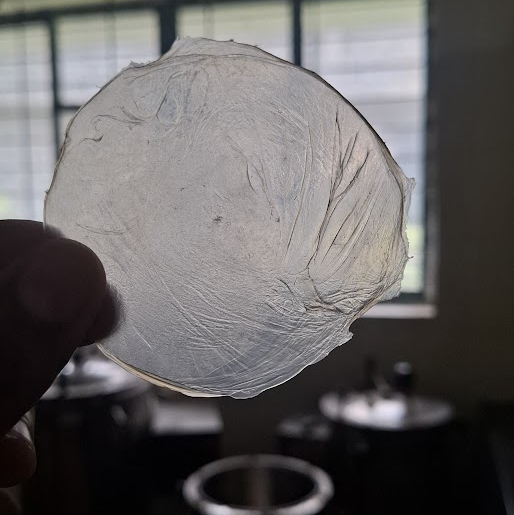
\includegraphics[width=\textwidth]{Figures/aquatrack/image2}
\caption{Prototype of the functional sodium alginate sweat patch}
\label{fig:functional-patch}
\end{minipage}
\hfill
\begin{minipage}{0.48\textwidth}
\centering
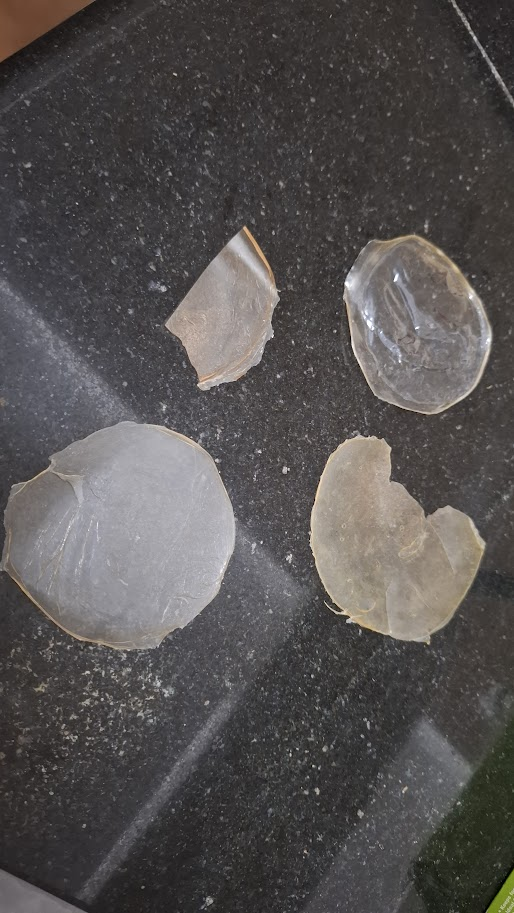
\includegraphics[width=\textwidth]{Figures/aquatrack/image3}
\caption{Functional sweat patches produced during sodium alginate trials}
\label{fig:functional-patches}
\end{minipage}
\end{figure}

\clearpage

\section{Swelling Ratio Analysis}

The swelling ratio of the sodium alginate hydrogel was calculated using:
\begin{equation}
\label{eq:swelling-ratio}
Swelling\ Ratio = \frac{W_{wet} - W_{dry}}{W_{dry}} \times 100
\end{equation}

For the tested patch, the wet weight was 0.9 g and the dry weight was 0.406 g. Substituting these values gives:
\begin{equation}
\label{eq:swelling-result}
Swelling\ Ratio = \frac{0.9 - 0.406}{0.406} \times 100 = 121.67\%
\end{equation}

The hydrogel therefore absorbed water and increased by approximately 122\%. This indicates moderate water-holding capacity, dense cross-linking, high mechanical strength, and the ability to entrap urease within the polymer network.

\begin{figure}[htb]
\centering
\begin{minipage}{0.48\textwidth}
\centering
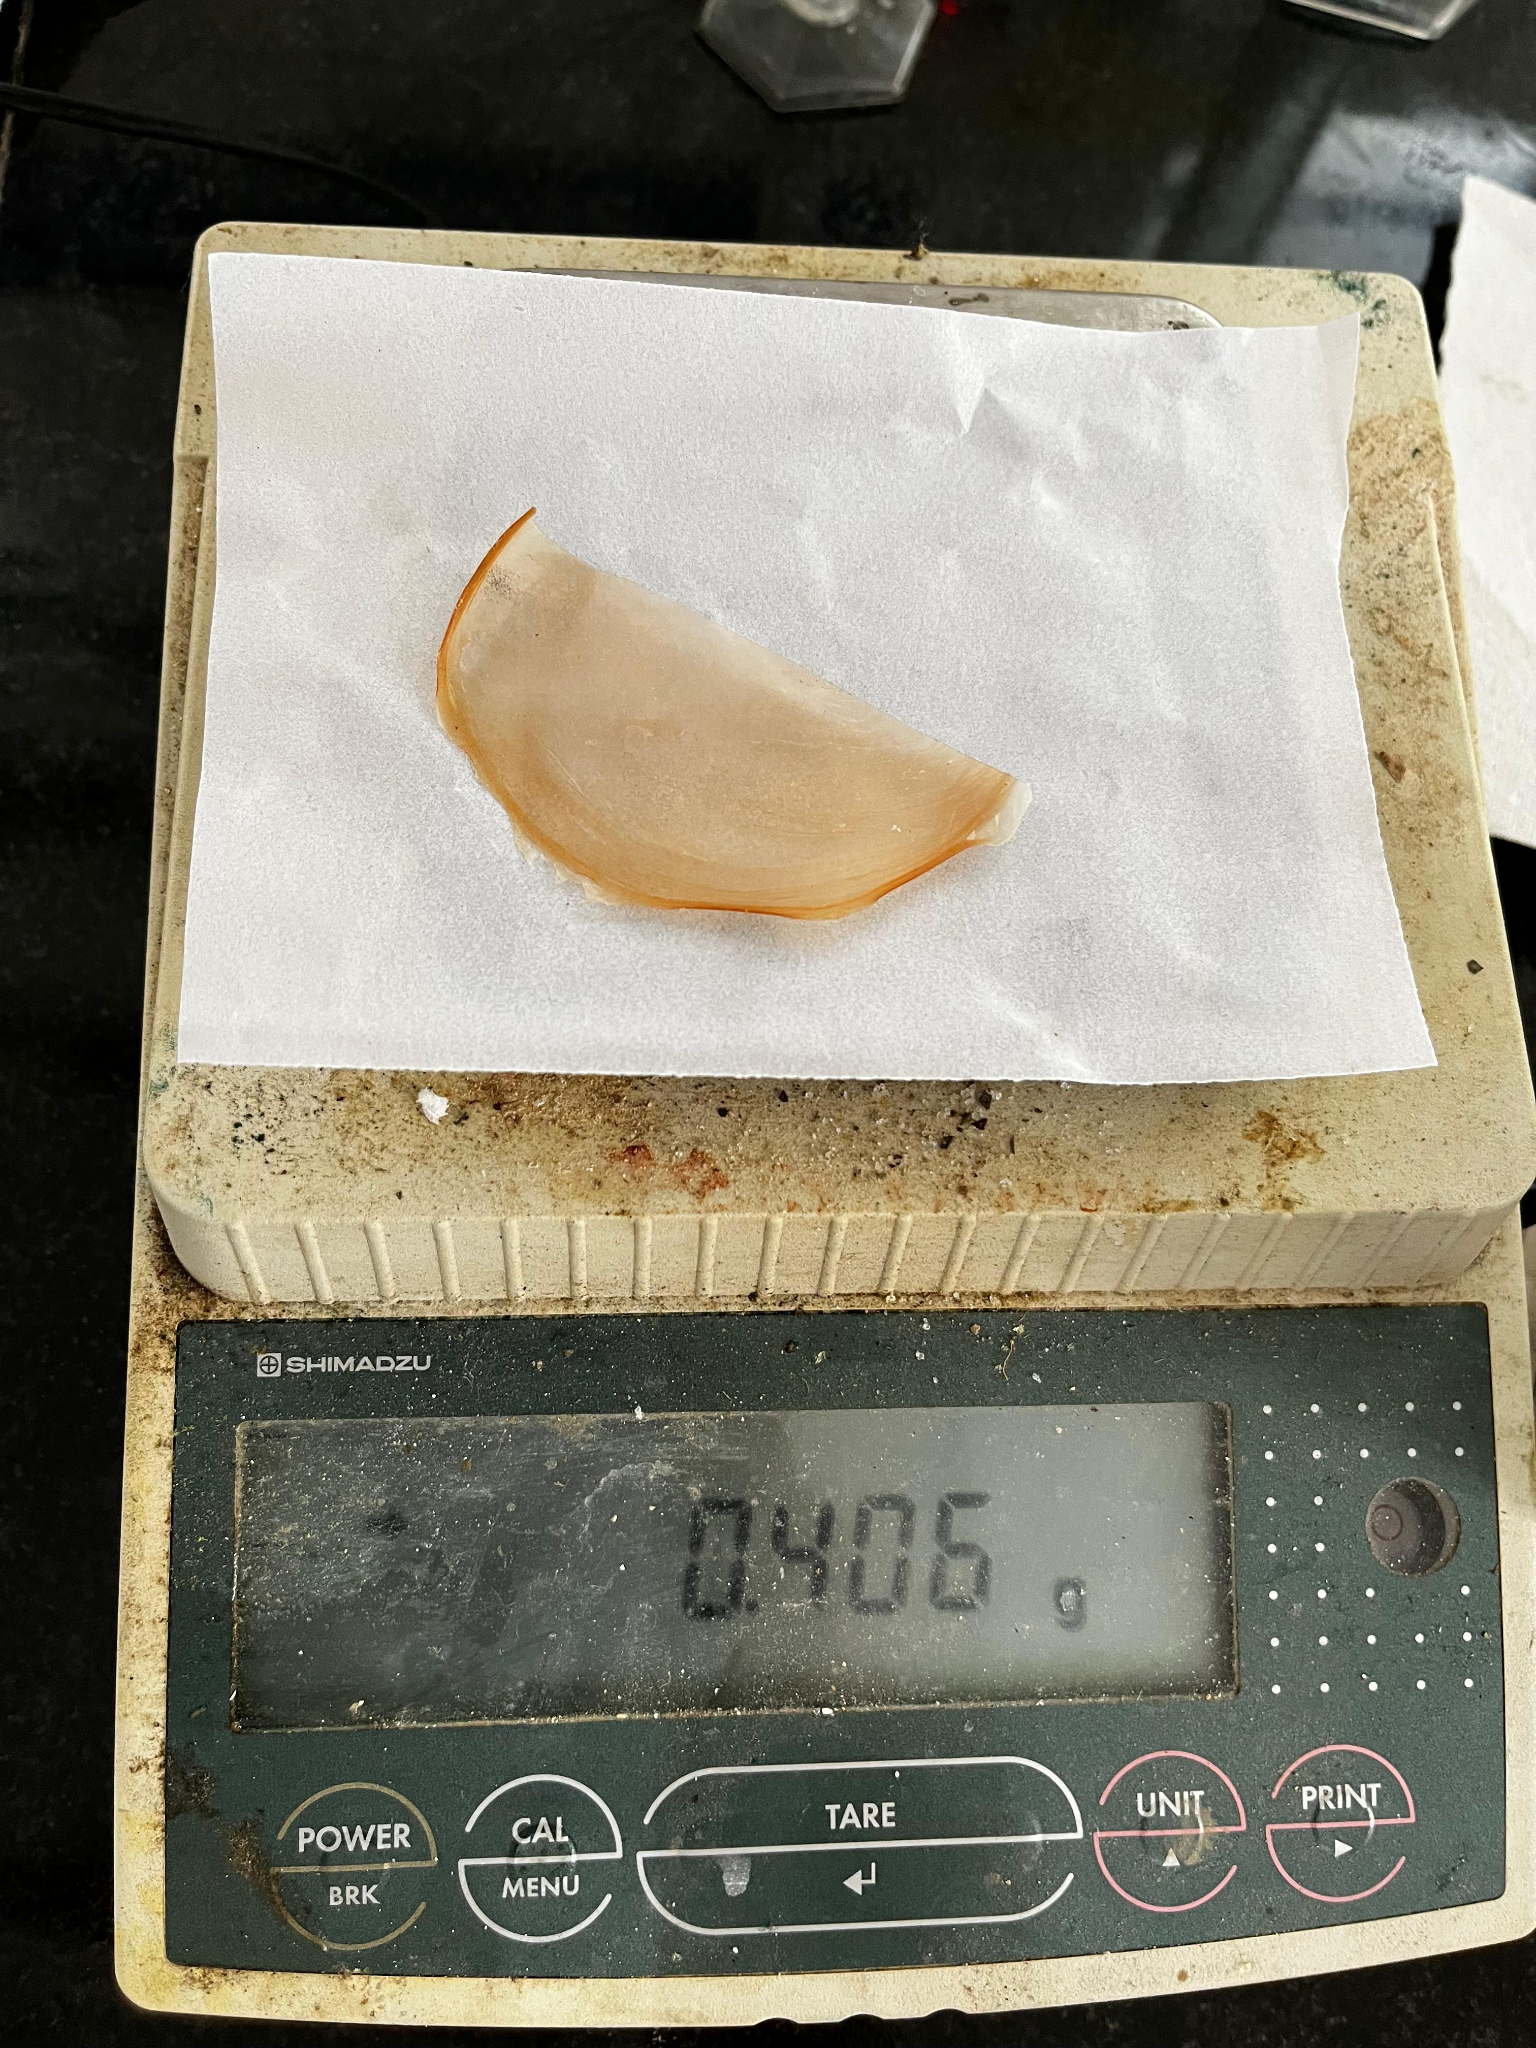
\includegraphics[width=\textwidth]{Figures/aquatrack/image10}
\caption{Dry weight measurement of the hydrogel patch}
\label{fig:dry-weight}
\end{minipage}
\hfill
\begin{minipage}{0.48\textwidth}
\centering
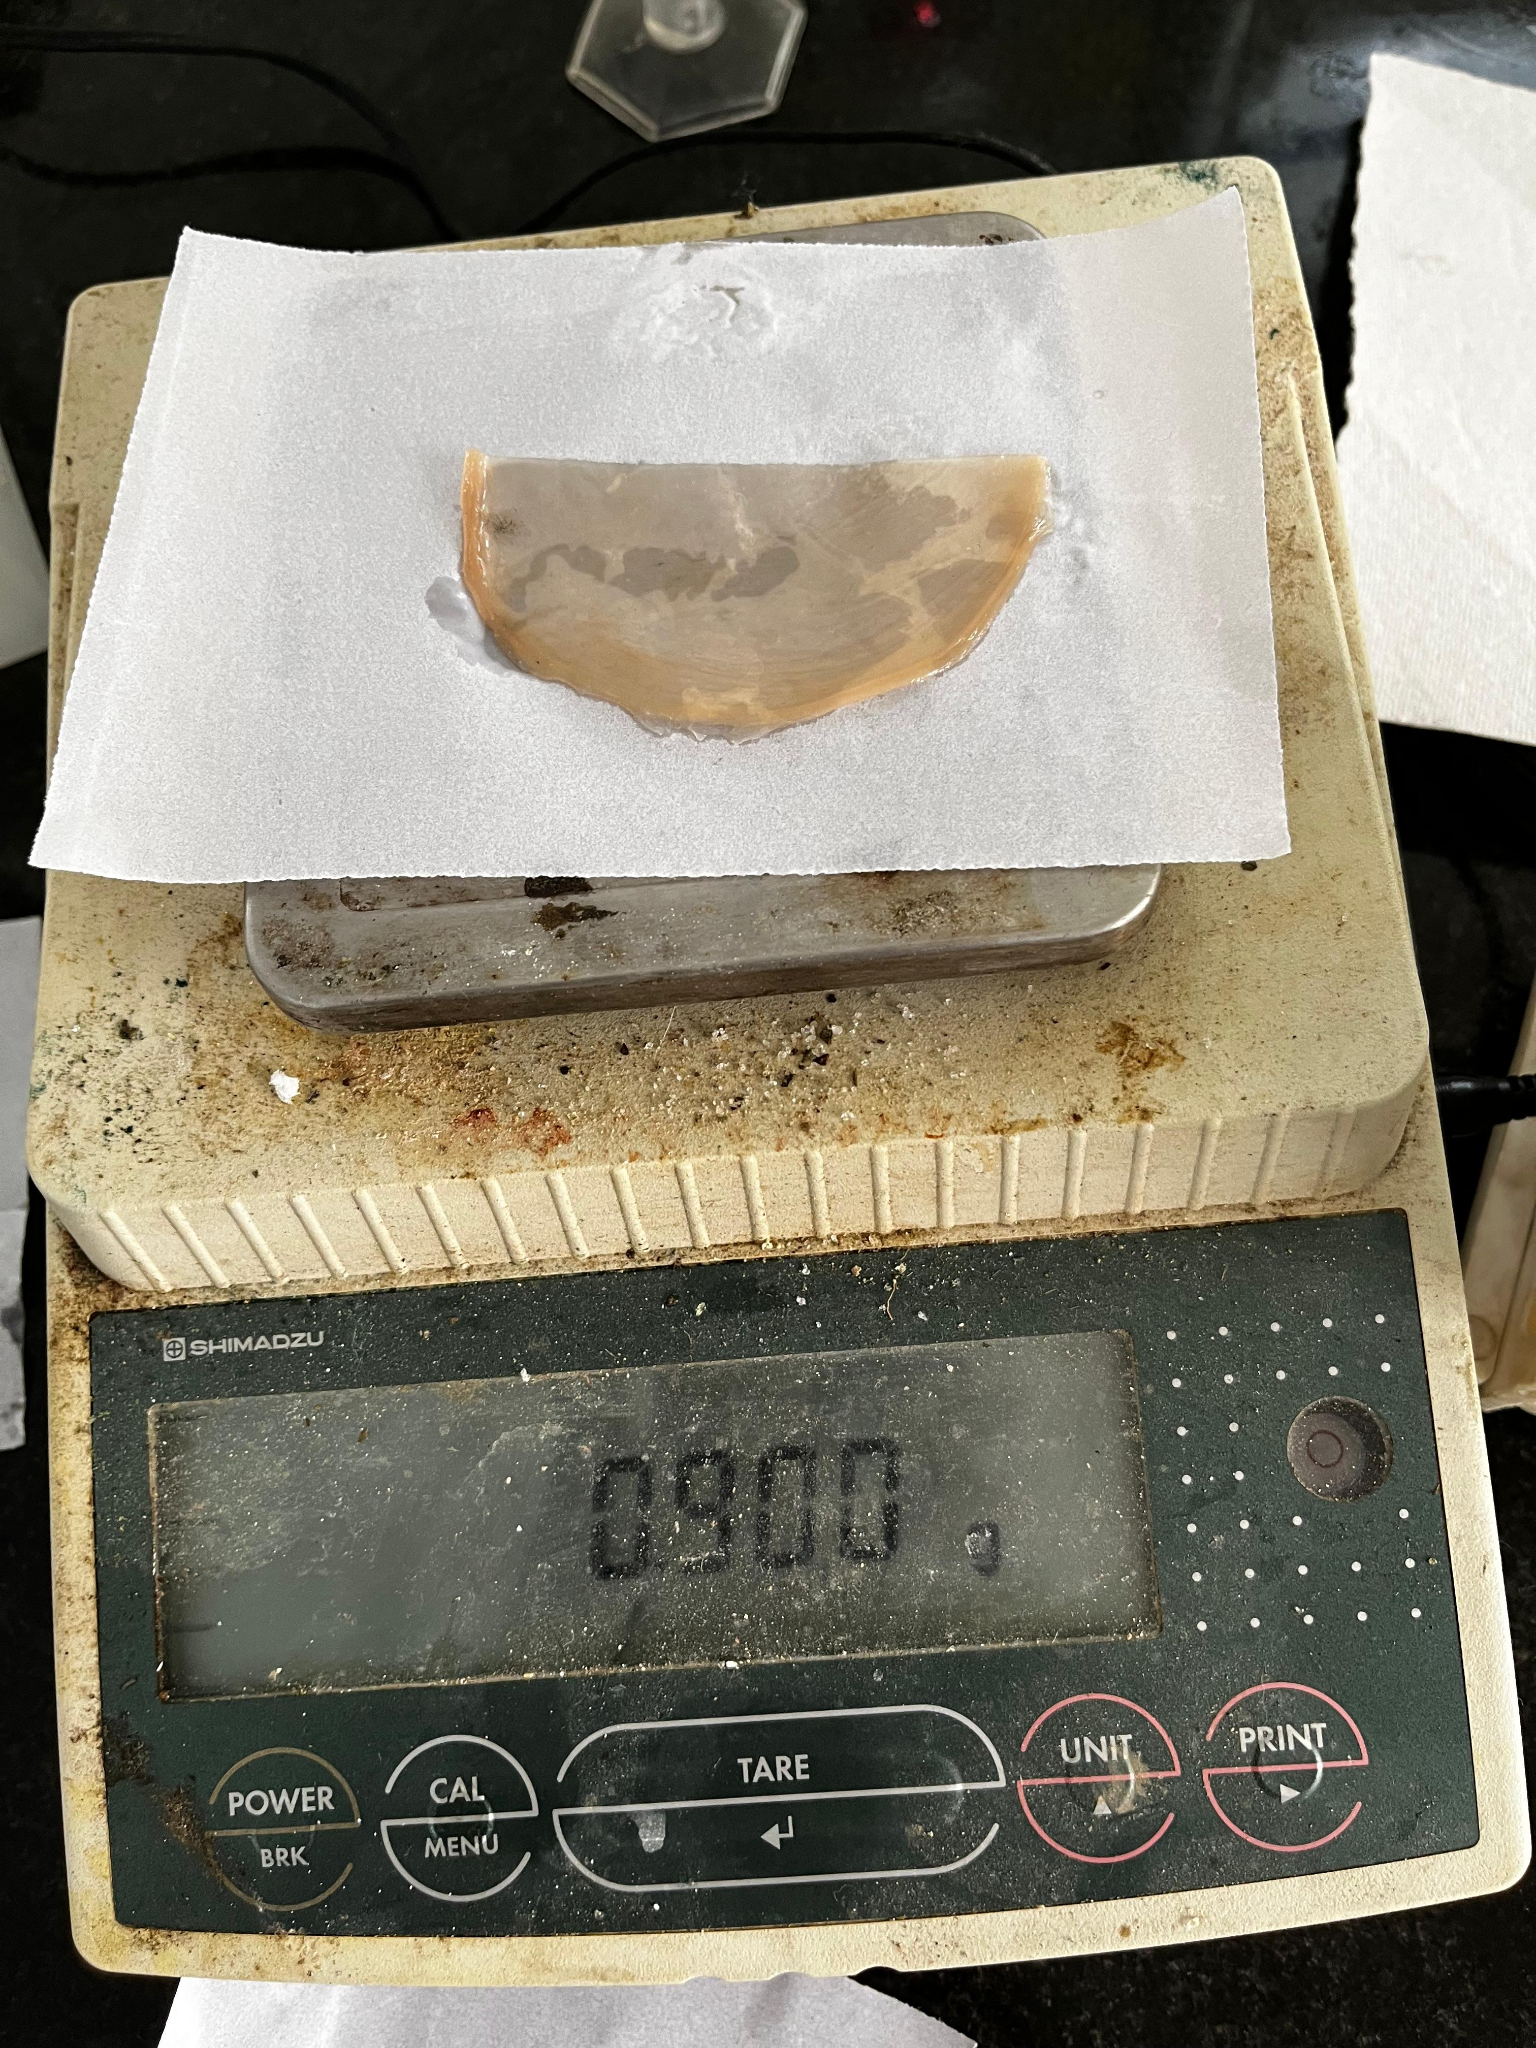
\includegraphics[width=\textwidth]{Figures/aquatrack/image8}
\caption{Wet weight measurement of the sweat patch}
\label{fig:wet-weight}
\end{minipage}
\end{figure}

\clearpage

\section{Colorimetric Assay}

The synthesized sodium alginate and PVA hydrogels were tested for urease activity using pH-dependent colorimetric response. Artificial sweat with elevated urea concentration was prepared to mimic the sweat chemistry expected in severe CKD conditions. Normal sweat is mildly acidic, typically around pH 4.0--6.8. When urea-rich sweat enters the hydrogel, immobilized urease hydrolyzes urea into ammonia. Ammonia increases local alkalinity, causing phenol red to shift toward a bright pink color. The intensity of the pink response indicates the strength of the urea exposure.

\begin{figure}[H]
\centering
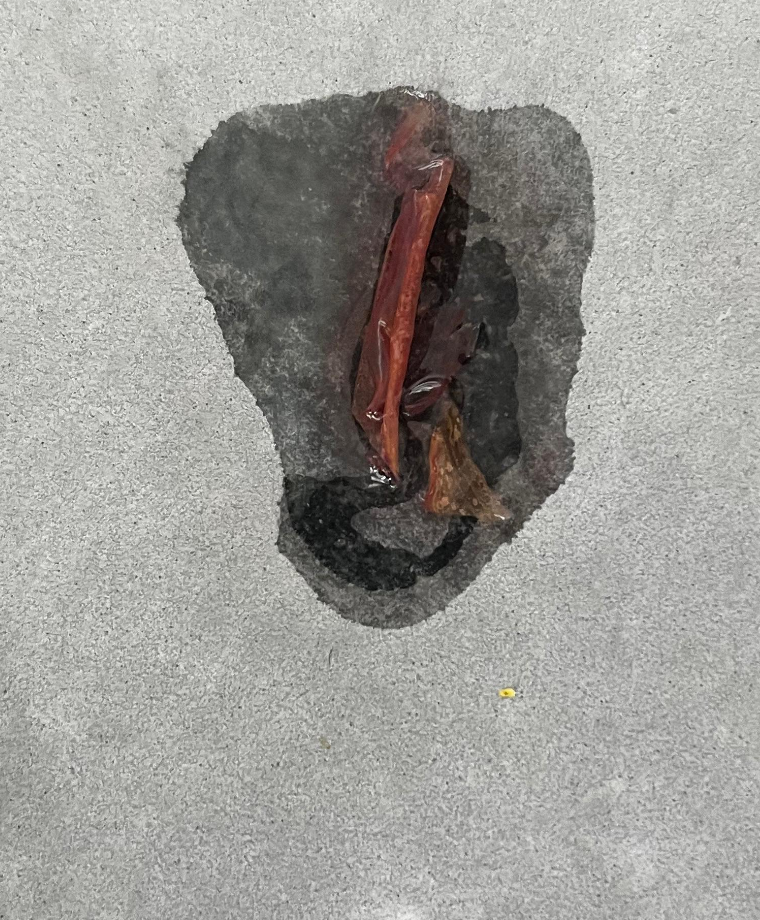
\includegraphics[height=0.42\textheight,keepaspectratio]{Figures/aquatrack/image11}
\caption{Color change of sodium alginate hydrogel after exposure to urea}
\label{fig:alginate-urea-color}
\end{figure}

\clearpage

\section{Time-Series Color Change Analysis}

For image-based response analysis, air-dried PVA patches were exposed to a standard urea concentration gradient from 0 to 100 mM. The sequence was captured at one-minute intervals to observe the gradual shift toward pink intensity, which indicates urease activity and increasing alkalinity due to ammonia formation.

\begin{figure}[H]
\centering
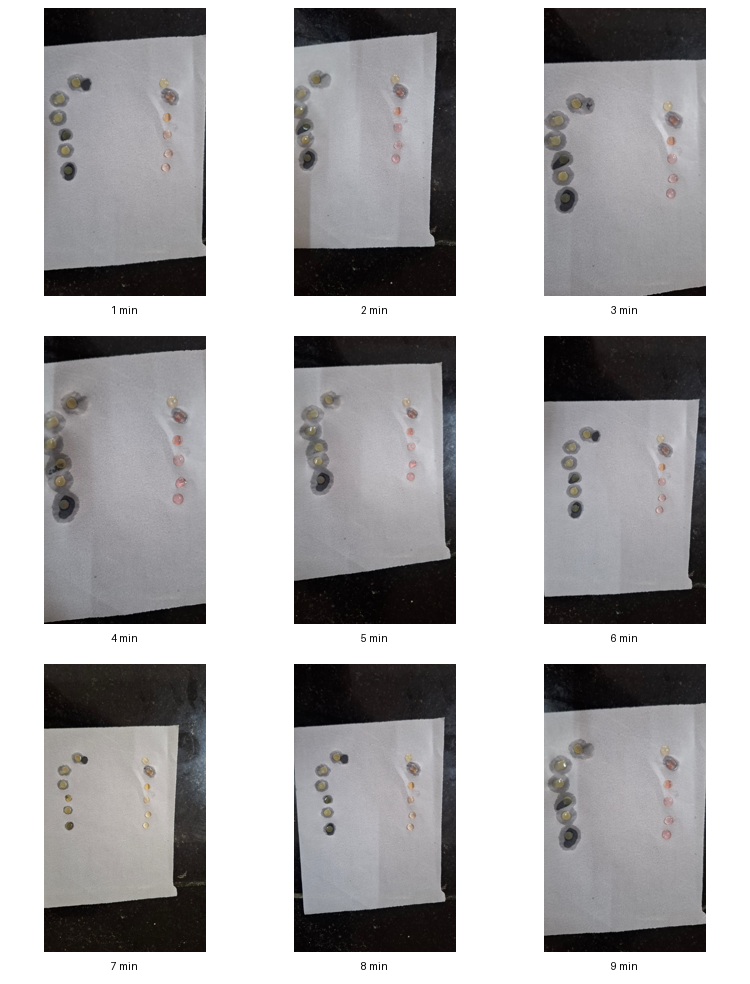
\includegraphics[height=0.65\textheight,keepaspectratio]{Figures/aquatrack/image16}
\caption{Representative time-series color change of PVA hydrogel}
\label{fig:pva-urea-gradient}
\end{figure}

\clearpage

\section{Classifier Performance}

\begin{figure}[!ht]
\centering
\begin{minipage}{0.48\textwidth}
\centering
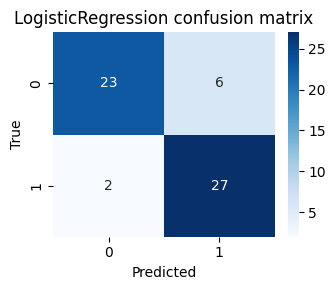
\includegraphics[width=\textwidth]{Figures/aquatrack/image12}
\caption{Confusion Matrix: Logistic Regression}
\label{fig:cm-lr}
\end{minipage}
\hfill
\begin{minipage}{0.48\textwidth}
\centering
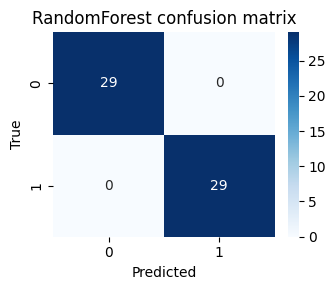
\includegraphics[width=\textwidth]{Figures/aquatrack/image13}
\caption{Confusion Matrix: Random Forest}
\label{fig:cm-rf}
\end{minipage}

\vspace{0.5cm}

\begin{minipage}{0.48\textwidth}
\centering
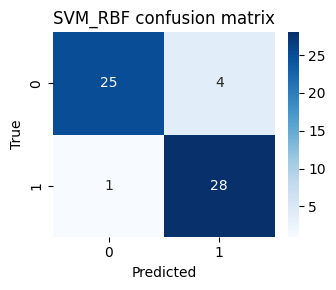
\includegraphics[width=\textwidth]{Figures/aquatrack/image14}
\caption{Confusion Matrix: SVM (RBF)}
\label{fig:cm-svm}
\end{minipage}
\hfill
\begin{minipage}{0.48\textwidth}
\centering
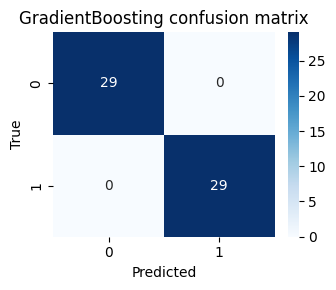
\includegraphics[width=\textwidth]{Figures/aquatrack/image15}
\caption{Confusion Matrix: Gradient Boosting}
\label{fig:cm-gb}
\end{minipage}
\end{figure}

Figures \ref{fig:cm-lr}--\ref{fig:cm-gb} show the confusion matrices for each of the available classifiers across different risk levels. In the biomarker pipeline, Logistic Regression achieved the highest cross-validation macro-F1 score of 0.9622 and a held-out test F1 score of 1.000 on 18 test samples. 

In the context pipeline, Random Forest and Gradient Boosting jointly achieved the highest cross-validation F1 score of 0.9957 and a held-out test F1 score of 1.000 on 58 test samples. Table \ref{tab:classifier-comparison} summarizes the quantitative performance metrics for both pipelines.

\begin{table}[htb]
\fontsize{10}{12}\selectfont
\centering
\caption{Classifier comparison across both pipelines}
\label{tab:classifier-comparison}
\begin{tabular}{|p{3.4cm}|c|c|c|c|}
\hline
\textbf{Classifier} & \textbf{$D_{main}$ CV F1} & \textbf{$D_{main}$ Test F1} & \textbf{$D_{ctx}$ CV F1} & \textbf{$D_{ctx}$ Test F1}\\
\hline
Logistic Regression & 0.9622 & 1.000 & 0.8697 & 0.8710\\
\hline
Random Forest & 0.8396 & 1.000 & 0.9957 & 1.000\\
\hline
SVM (RBF) & 0.9210 & 0.9850 & 0.9360 & 0.9180\\
\hline
Gradient Boosting & 0.9050 & 0.9520 & 0.9957 & 1.000\\
\hline
\end{tabular}
\end{table}

\begin{table}[htb]
\small
\centering
\caption{Distribution of weighted fusion score across derived risk classes.}
\label{tab:fusion-score-dist}
\begin{tabular}{lcccc}
\toprule
\textbf{Risk Class} & \textbf{n} & \textbf{Mean F} & \textbf{Min F} & \textbf{Max F} \\
\midrule
Low & 30 & 0.203 & 0.096 & 0.243 \\
Medium & 30 & 0.295 & 0.247 & 0.351 \\
High & 30 & 0.471 & 0.354 & 0.744 \\
\bottomrule
\end{tabular}
\end{table}

\section{Discussion}

The results indicate that the AquaTrack architecture is feasible at both the sensing and computational levels. The sodium alginate hydrogel provides a practical and flexible medium for sweat collection and urea-responsive colorimetric detection. The machine learning pipeline demonstrates that biomarker features and context features can be modeled independently and then fused to improve interpretability.

The perfect test scores should be interpreted carefully because the datasets are relatively small and the labels are derived rather than clinically annotated. However, the high cross-validation scores show that the engineered features are internally consistent and that the dual-pipeline design is promising for future validation on larger real-world datasets.

The context pipeline adds value by identifying conditions where the biomarker-only prediction may require correction. This is important for mobile health use because sweat availability, exertion, and climate can influence sensor readings. A fused prediction score therefore provides a more practical decision layer than a single model output. The statistical distribution of these scores across the predicted risk categories is presented in Table \ref{tab:fusion-score-dist}, which validates the score separability and clinical alignment of the framework.
